\section{Introduction to RAG and the CRAG benchmark}
\label{sec:intro}
The rise of Large Language Models (LLMs) has revolutionized the field of natural language processing~\cite{yasunaga-etal-2021-qa,liu2023pre,lievin2024can,statsqa}, but these models still struggle with providing accurate and reliable answers to complex questions. One major challenge is the tendency for LLMs to ``hallucinate'' or generate responses that are not grounded in factual information~\cite{rawte2023troubling, 10.1145/3571730,sun2024large,verifai}. To address this issue, researchers have turned to Retrieval-Augmented Generation (RAG)~\cite{gao2024ragsurvey,lewis2021retrievalaugmented,chen2023benchmarking,symphony}, a technique that involves searching external sources to gather relevant information and then using that information to generate more accurate answers (Figure~\ref{fig:rag}).

\begin{figure}[h]
  \centering
  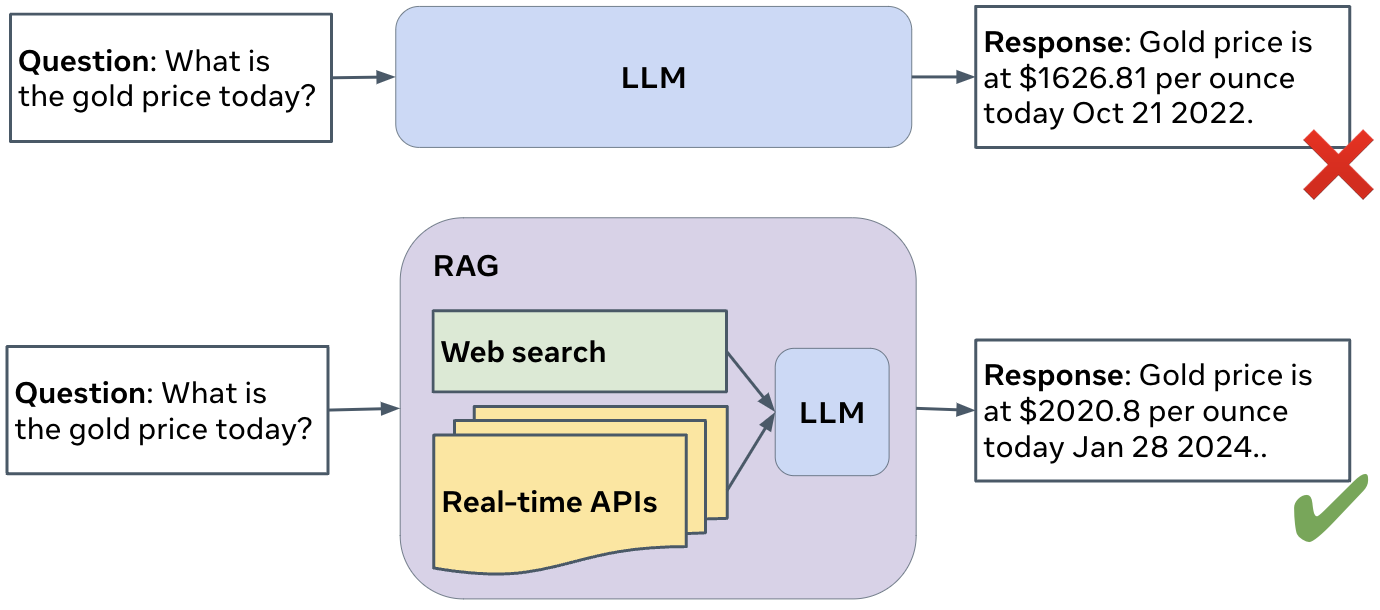
\includegraphics[width=12cm]{submissions/Xiao2024/figs/RAG.png}
  \caption{Given a question, a RAG system searches external sources to retrieve relevant information and then provides grounded answers.}
  \label{fig:rag}
\end{figure}

However, existing datasets for evaluating RAG systems are limited in their scope and diversity, failing to capture the complexity and nuance of real-world question-answering tasks. To address this limitation, we developed the Comprehensive RAG (CRAG) Benchmark, a comprehensive evaluation framework designed to assess the capabilities of RAG systems. The benchmark comprises over 4.4K question-answer pairs, accompanied by mock APIs that mimic the process of searching the web and accessing knowledge graphs. 
CRAG is across five domains (finance, sports, music, movie, and encyclopedia open domain), and a diverse range of question types, including simple-fact questions, questions that require aggregation and reasoning. 
CRAG further encompasses varied entity popularity from popular to long-tail and temporal spans ranging from seconds to years. As such, it covers a broad spectrum of real user queries, providing a realistic and challenging testbed for RAG systems~\cite{yang2024crag}. By incorporating both web and knowledge graph search, CRAG simulates realistic information retrieval scenarios, reflecting the common practice of users seeking answers from multiple sources. 
Our evaluations using this benchmark revealed substantial performance gaps in even the most advanced LLMs and RAG systems, highlighting the need for continued research and development in this area.

The CRAG benchmark served as the foundation for the KDD Cup 2024 competition, which drew over 2.5K participants and 5.6K submissions from around the world. The winning solutions demonstrated significant improvements over baseline methods. In this paper, we present key insights and takeaways from the competition, including our learnings on the RAG landscape (Section~\ref{sec:raglandscape}), learnings from the CRAG winning solutions (Section~\ref{sec:winning-solutions}), and learnings from hosting the CRAG challenge (Section~\ref{sec:hosting}), suggesting directions for future RAG research.

%\subsection{The CRAG benchmark}
%\label{sec:crag_benchmark}

